%%%%%%%%%%%%%%%%%%%%%%%%%%%%%%%%%%%%%%%%%%%%%%%%%%%%%%%%%%%%%%%%%%%%%%%%%%%%%%%%
%2345678901234567890123456789012345678901234567890123456789012345678901234567890
%        1         2         3         4         5         6         7         8

% Key links for ICRA2020
% CFP: https://www.icra2020.org/call-for-papers
% PaperPlaza: https://ras.papercept.net/conferences/scripts/start.pl
% Author Guidelines: http://ras.papercept.net/conferences/support/tex.php

\documentclass[letterpaper, 10 pt, conference]{ieeeconf}
%\documentclass[a4paper, 10pt, conference]{ieeeconf}

% This command is only needed if you want to use the \thanks command
\IEEEoverridecommandlockouts

\overrideIEEEmargins

%In case you encounter the following error:
%Error 1010 The PDF file may be corrupt (unable to open PDF file) OR
%Error 1000 An error occurred while parsing a contents stream. Unable to analyze the PDF file.
%This is a known problem with pdfLaTeX conversion filter. The file cannot be opened with acrobat reader
%Please use one of the alternatives below to circumvent this error by uncommenting one or the other
%\pdfobjcompresslevel=0
%\pdfminorversion=4

% See the \addtolength command later in the file to balance the column lengths
% on the last page of the document

\usepackage{amsmath}
\usepackage{amssymb}
\usepackage{bm}
\usepackage{textcomp}
\usepackage{gensymb}
\usepackage{graphicx}
\usepackage{tabularx}
\usepackage{array}
\usepackage{booktabs}
\usepackage{subcaption}

\captionsetup[table]{
    justification=centerlast,
    textfont=small,
}

\graphicspath{{figures/}}

% Set a style for an entire table row
\newcolumntype{$}{>{\global\let\currentrowstyle\relax}}
\newcolumntype{^}{>{\currentrowstyle}}
\newcommand{\rowstyle}[1]{\gdef\currentrowstyle{#1}%
    #1\ignorespaces
}

% Some small icons we use in the text
\newcommand{\com}{\,
\includegraphics[width=9pt]{ico-com}\,}
\newcommand{\hinge}{\,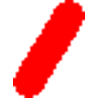
\includegraphics[width=9pt]{ico-hinge}\,}
\newcommand{\motor}{\,
\includegraphics[width=9pt]{ico-motor}\,}

\usepackage{lipsum}

\title{
    \LARGE \bf%
    A Reduced-Order Approach to Assist with Reinforcement Learning for Underactuated Robotics
}

\author{
    J\'er\'emy Augot$^{1,2}$, Aaron J. Snoswell$^{2}$ and Surya P. N. Singh$^{2}$
    % <-this % stops a space
    \thanks{
        $^{1}$Ecole CentraleSup\'elec, Paris, France
    }%
    \thanks{
        $^{2}$The Robotics Design Lab at The University of Queensland, Brisbane, Australia
    }%
}

\begin{document}

\maketitle
\thispagestyle{empty}
\pagestyle{empty}

%%%%%%%%%%%%%%%%%%%%%%%%%%%%%%%%%%%%%%%%%%%%%%%%%%%%%%%%%%%%%%%%%%%%%%%%%%%%%%%%
\begin{abstract}

\lipsum[1]

\end{abstract}

%%%%%%%%%%%%%%%%%%%%%%%%%%%%%%%%%%%%%%%%%%%%%%%%%%%%%%%%%%%%%%%%%%%%%%%%%%%%%%%%
\section{INTRODUCTION}

As robots become more compliant and variable they become more capable, and more complex.  Underactuated robots, for example, provide great design freedom, yet their adoption has been limited by the need for manual controller designs.

Deep Reinforcement Learning (DRL) methods offer automated tools for robotic control by identifying a policy that maximize the expected sum of rewards \cite{henderson2018deep}.  This has been extended to continuous control domains via algorithms such as the Deep Deterministic Policy Gradient (DDPG) \cite{DDG}, Proximal Policy Optimization (PPO) \cite{PPO}, Soft Actor-Critic (SAC) \cite{SAC}, and Twin Delayed Deep Deterministic (TD3) \cite{TD3}.  The power of these methods comes, in part, from the high-dimensional, nonlinear function approximation of both the policy and the expected value via neural networks.  The dimensionality of this rich representations also presents a challenge for sample collection, stability, and convergence \cite{Islam2017}.  Reducing the order seems an natural approach to addressing this challenge, but doing so directly requires carefully defining suitable (state-space) features as the aforementioned methods are sensitive to the chosen representation \cite{bhatnagar2009convergent}.  

Interestingly, many robots are underactuated by design, or at times, by circumstance (e.g., due to motor saturation).  Such systems achieve their tasks due to the inherent dependence of their actuation states.  This implicit structure suggests that an (automatic) reduction of the actuation space to a would be make these systems more compatible with (model-free) DRL methods; and would allow more variable underactuated systems.  Towards this, we introduce a highly variable, single actuator robotic locomotion benchmark based around a passive compliant toy system (see also Fig. \ref{fig:one}).

The contributions of this paper are ...
We present a reduced order variant for this domain.
We introduce the Jitterbug Problem as a diverse underactuated robotics task with dynamic, compliant and non-trivial motion in five scenarios of varying gradations of task complexity. 
And, we find that reduced order models can have similar (reward) performance, yet empirically have less training variance and slightly better learning rates.







% In the case of robhot


% , which, if not done careful 

% this directly requires physical models and is challenging when there is high variance or uncertainty.   



% Underactuated robots, in particular, are compatible with this notion for the 

%  other aspect that 





% Underactuated robots naturally 

% are such a system.  



% These also represent a curse in that 


%  flexibility in representing  

% In general, a challenge to using these methods


% The use of DRL  In general, a challenge for these  these cases has 



% %by identifying the ``best'' policy and

% Model-free 

% and has shown promising results in a variety of robotic tas  




% such as the 



% trial and error, but have been limited by the   
 


% but they 

% for continuous control, such as DDPG 




% Underactuated robots are a class of such systems that provide the designer great options, but have been limited 




% One of the challenges with these methods is handing high dimensional 

Foo bar \cite{Haarnoja2018SAC}






\lipsum[1-2]

\begin{figure}[ht]
    
    \centering
    
    \begin{minipage}[b]{0.49\linewidth}
        \centering
        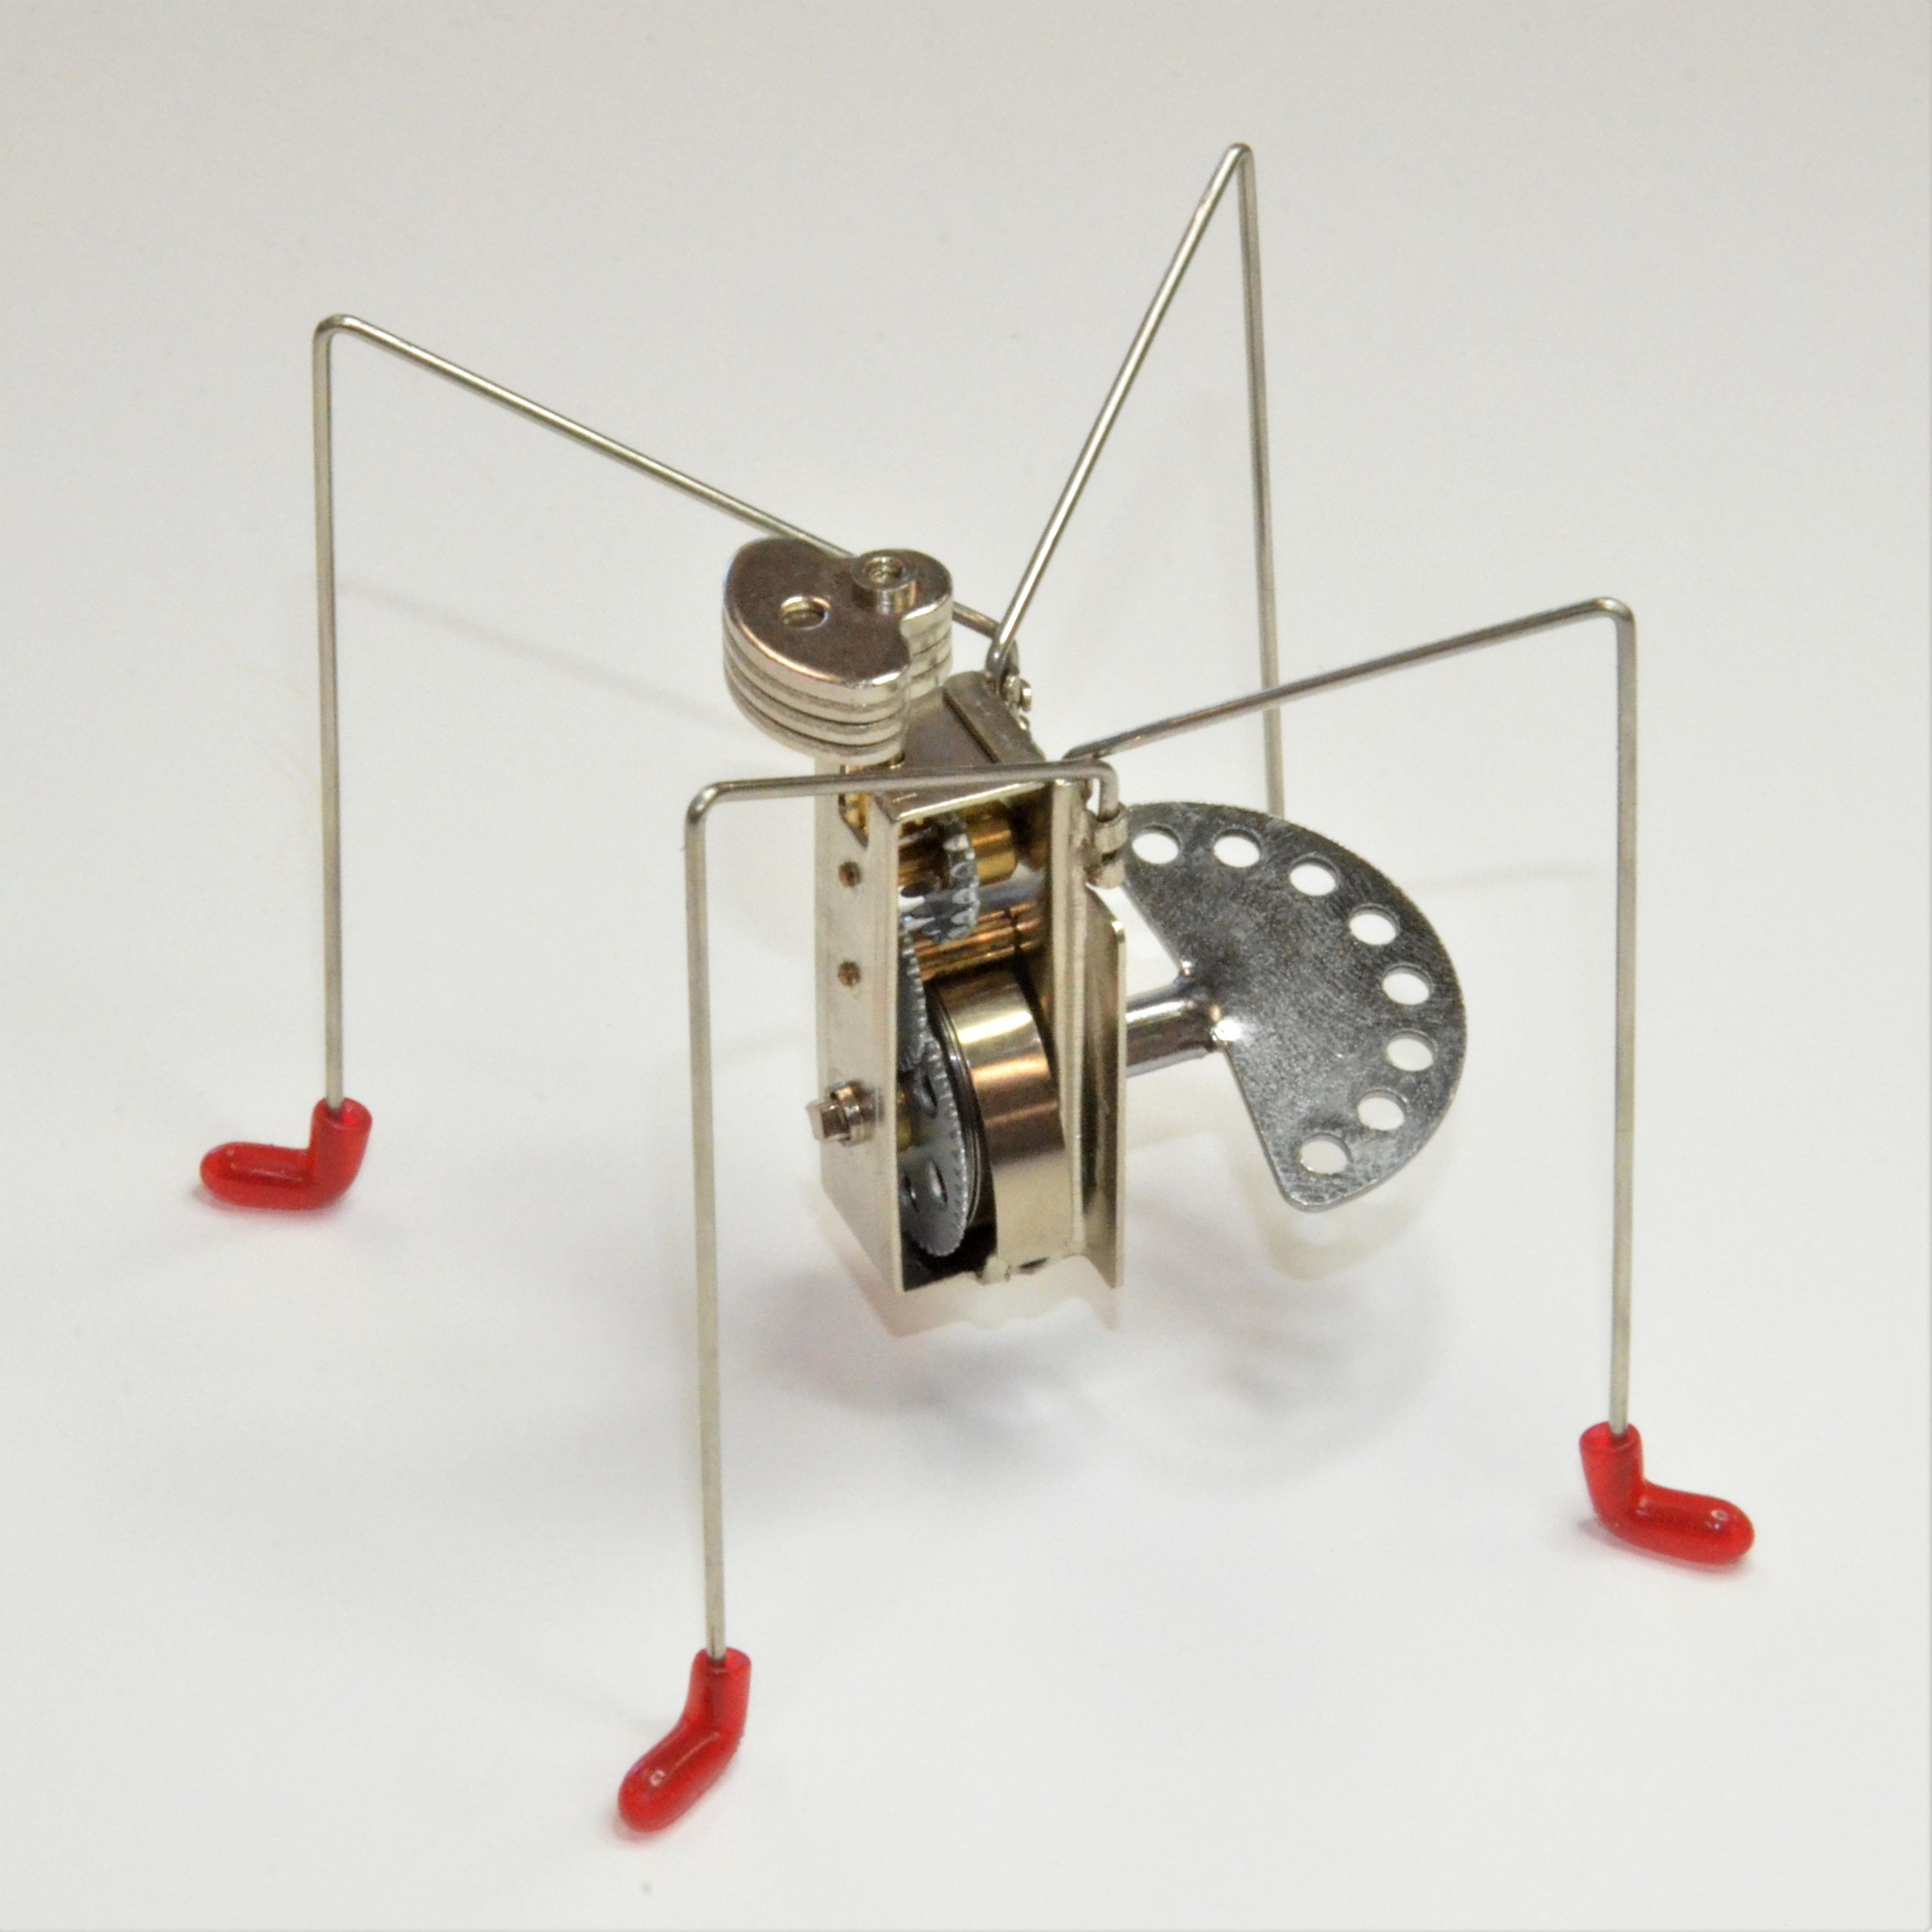
\includegraphics[width=\linewidth]{katita}
    \end{minipage}
    \begin{minipage}[b]{0.49\linewidth}
        \centering
        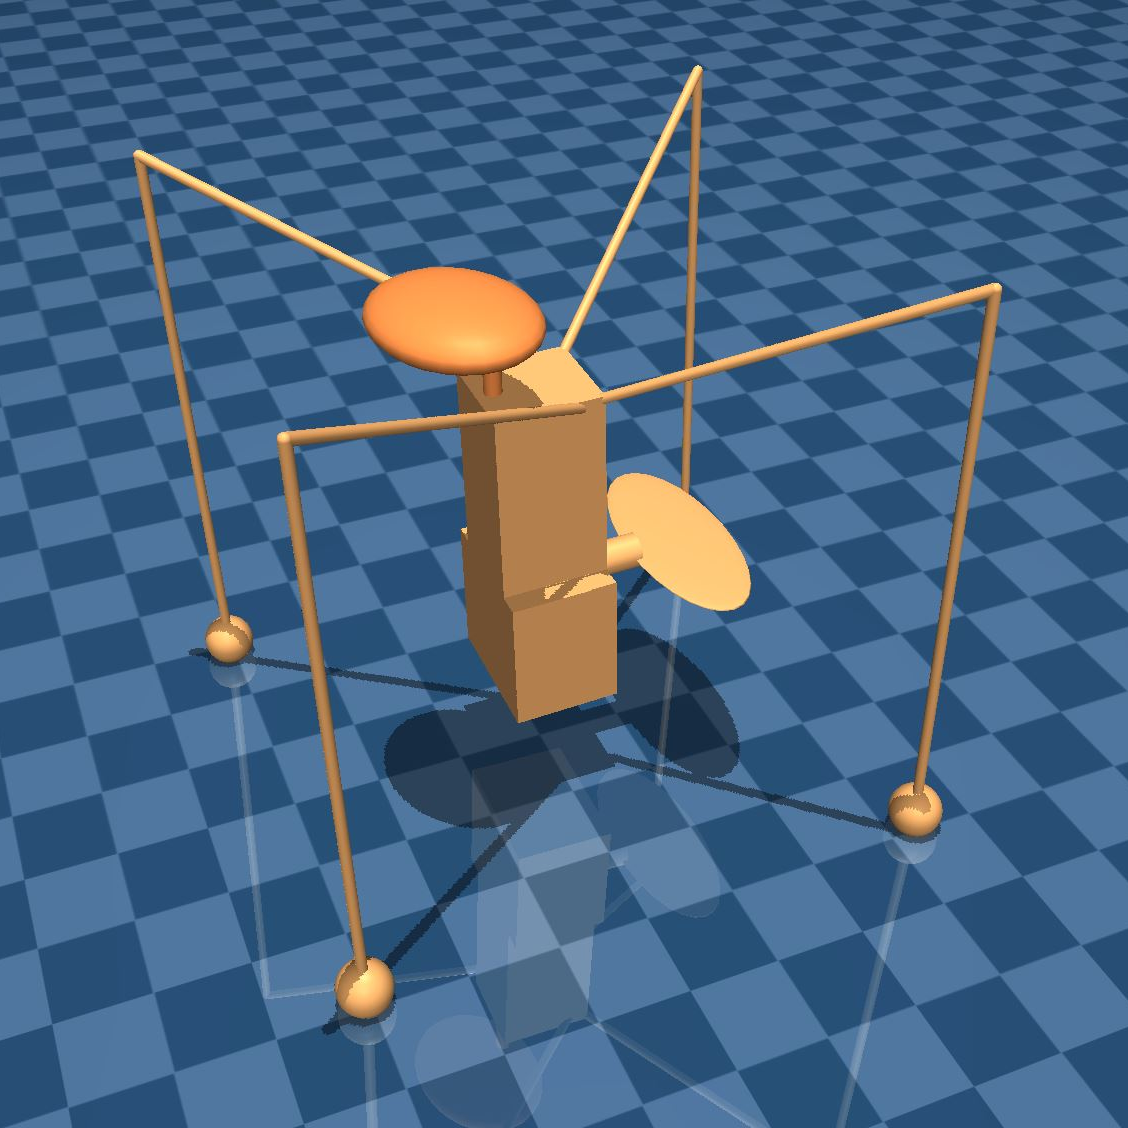
\includegraphics[width=\linewidth]{jitterbug}
    \end{minipage}
    
    \caption{
        The wind-up children's toy `Katita' (left) was the inspiration for our underactuated `Jitterbug' continuous control task (right).
        In the simulated robot the wind-up spring is replaced with a controlled single degree-of-freedom motor.
        %The simulated robot retains the (non functional) wind-up crank to more closely mimic the mass distribution of the real toy.
        For scale, the blue checks on the simulated floor on the right are 1cm in size.
    }
    \label{fig:leader}
    
\end{figure}

\lipsum[1-4]

\section{RELATED WORK}


Reinforcement Learning is an ....  



Reinforcement Learning (RL) methods offer automated tools for controller design of such systems via trail and error \cite{sutton1998reinforcement}, but have been been limited by feature representations and forward models \cite{duan2016benchmarking}.  Deep Reinforcement Learning (DRL) algorithms for continuous control address this through the use of deep neural networks for both the policy ("actor") and value function ("critic") \cite{DDPG, SAC}.  Such systems have been  


\subsection{Deep Reinforcement Learning}


and have shown promise in a host of challenging applications including visualmotor learning \cite{finn2016deep} and VR teleoperation \cite{zhang2018deep}. 

%\subsection{Deep Deterministic Policy Gradients (DDPG)}

%\subsection{Advantage Actor-Critic (A2C)}

%\subsection{Proximal Policy Optimization (PPO)}

%\subsection{DeepMind Control Suite}

%\subsection{Under-actuated Control}


\subsection{Reduced Order Approaches for Underactuated Robotics}

Underacted robots are fundamentally correlated in their actuation space  \cite{tedrake2009underactuated}.  When a model is available control strategies ranging from optimal control \cite{betts2010practical} to direct collocation \cite{von1993numerical} to trajectory optimization \cite{kalakrishnan2011stomp} have been applied.  Some novel robots, such as compliant legged robots or soft robots, tend to exhibit complex dynamics that do stymie dynamical system and model reduction approaches as an explicit physical model may not be available \cite{nakajima2015information}.  Learning the model empirically, such as via a neural network, typically centers around obtaining a model that forecasts the robot's next timestep which is then used subsequently for control, such as via Model Predictive Control (MPC)  for a legged robot \cite{nagabandi2018learning} or for manipulation with a soft-gripper \cite{nishimura2017thin}.  

Highly variable motion is not random.  Given that actuation space for underactuated robots is structured, an autoencoder would be able to automatically discover some of these correlations \cite{AE_hinton2006reducing, ngsparse}.  A concern, however, is that the reduced model is not always intuitive, which would complicate the subsequent synchronization with a model based control strategy.   Model-free deep reinforcement learning (DRL) continuous control methods, however, are rather compatible with an autoencoder's reduced state description.

The use model reduction complements said DRL methods...
.... This has been considered for reinforcement learning ... 

This has been particularly effective in cases with very high dimensional inputs, such as from video, for low-dimensional independent constraints, such as obstacle locations \cite{finn2016deep, lynch2019learning}....



%\lipsum[1-2]

\begin{figure}[ht]
    \centering
    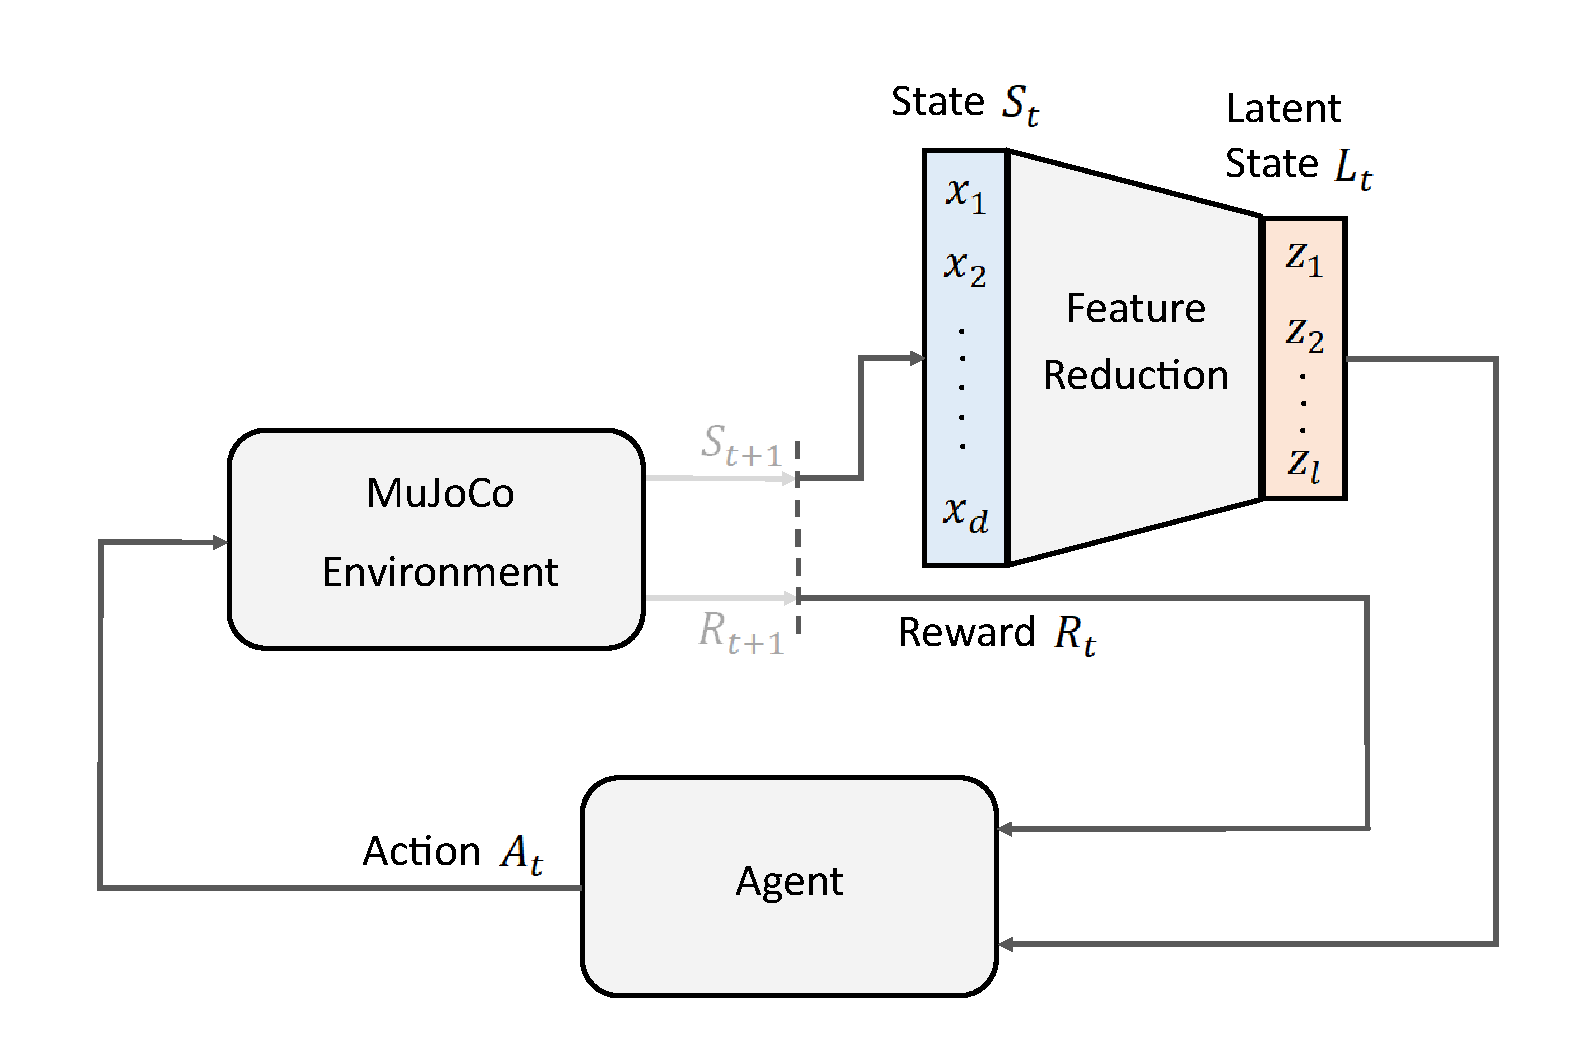
\includegraphics[width=\linewidth]{fig-system-arch}
    \caption{
        The architecture of our system.
    }
    \label{fig:system-arch}
\end{figure}

\section{METHOD}


We use the intuition that an underacted system has correlations between states %(otherwise it would be uncontrollable for said states)
and thus there is a lower-dimensional representation that could describe this process.  




\lipsum[1-9]

\section{A NOVEL, UNDER-ACTUATED CONTROL BENCHMARK}

We implemented our Jitterbug benchmark using the DeepMind Control Suite (DMC) framework [REF].
DMC is a framework and set of benchmark tasks for continuous control published by Google DeepMind in 2018.
DMC benchmarks consist of a \emph{domain} defining a robotic and environment model and \emph{tasks} which are instances of that domain with specific MDP structure

DMC uses the robust Multi-Joint dynamics with Contact (MuJoCo) robotics physics engine for simulation [REF].
To aid comparison across tasks, DMC imposes constraints on rewards ($R \in [0, 1]$) and episode length ($H = 1000$).
As such, for any DMC task, cumulative episode return $\approx 1000$ indicates success.

DMC tasks are compatible subsets of the popular OpenAI Gym framework [REF], meaning many popular RL algorithm frameworks can be used with these benchmarks.

\subsection{The Jitterbug Domain}

Our Jitterbug model was inspired by the children's toy Katita (Figure~\ref{fig:leader}).
We aimed to reproduce the physical dynamics of this toy while enabling control by replacing the wind-up spring with a single actuator of equivalent torque.
Our Jitterbug model conforms to the dimensions and mass of the Katita, however we replace the wind-up spring with a controlled single degree-of-freedom motor.
We retain the (non-functional) wind up crank to more closely model the mass distribution of the physical Katita.

We used high-speed recording and visual tachometry to measure the Katita motor speed and leg vibration modes.
By reverse-engineering the Katita gearbox we estimated the torque output of the drive spring and configured the MuJoCo actuator appropriately.
We modelled the legs as rigid bodies with shoulder and elbow hinge joints.
The hinge stiffness was manually tuned to reproduce the dominant leg vibration mode observed in our high-speed footage.
The Jitterbug model density was set using standard values for stainless steel ($7700$ kg/m$^3$) for the body and tough plastic ($1100$ kg/m$^3$) for the feet.
Figure~\ref{fig:parts} shows the physical composition of our simulated Jitterbug model.

\begin{figure}[ht]
    \centering
    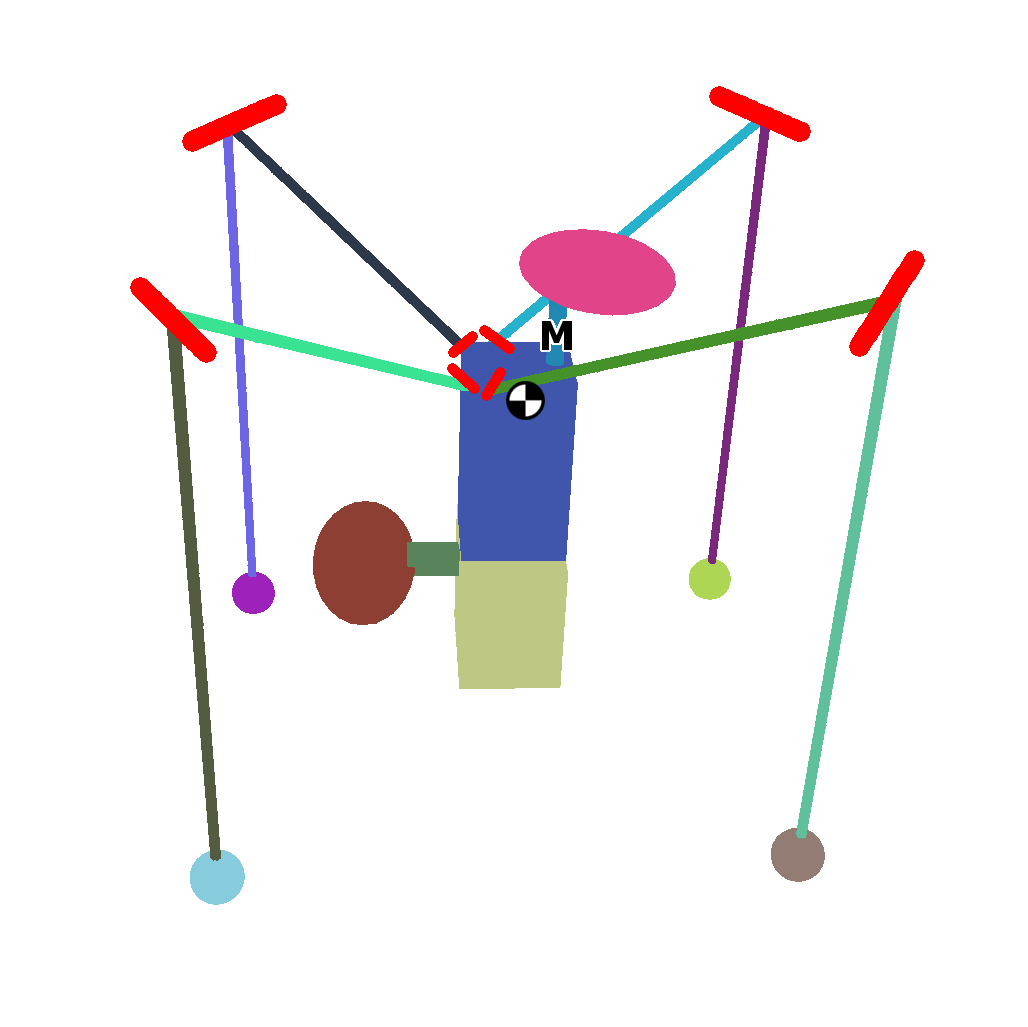
\includegraphics[width=\linewidth]{fig-jitterbug-parts}
    \caption[
        Schematic representation of the Jitterbug model.
        Individual rigid bodies are in different colours and we highlight the position of the center of mass, hinge joints and the single motor.
    ]{
        Schematic representation of the Jitterbug model.
        Individual rigid bodies are in different colours and we highlight the position of the center of mass (\protect\com), hinge joints  (\protect\hinge) and the single motor (\protect\motor).
    }
    \label{fig:parts}
\end{figure}

Due to the importance of contact and stiff dynamics in the Jitterbug's locomotion, we found it necessary to adjust MuJoCo's default settings, selecting an integration timestep of $0.0002$ and semi-implicit Euler integration.
With these settings we qualitatively observed a close correspondence between the Katita and the simulated dynamics under constant motor actuation on the Jitterbug.

DMC supports the definition of physically-based camera models for to enable learning from raw pixels if desired.
We defined several cameras for the Jitterbug domain including an overhead, tracking and ego-centric view.

\subsection{The Jitterbug Task Suite}

The Jitterbug dynamics naturally induce very high variance motion under a range of motor velocities.
We defined a collection of five tasks of increasing difficulty based on the Jitterbug domain.
The tasks were designed with increasingly sparse reward signals to increase the difficulty.

For all tasks we choose $\gamma = 0.99$ and consider a task solved when cumulative episode reward is $\gtrapprox 900$.
In all tasks the Jitterbug is reset to a random pose near the origin at the start of an episode.
All tasks have a single continuous action controlling the motor $\mathcal{A} = [-1, 1]$ (larger/smaller values are clipped) and continuous state and observation spaces.

For each task, we report ($\text{dim}(\mathcal{S}), \text{dim}(\mathcal{O})$) and a brief description of the reward structure.
Tasks are reported here ordered easiest to hardest.

\begin{enumerate}
    
    \item \emph{Move From Origin} (16, 15): The Jitterbug must move away from the origin in any direction.
    N.b. a sufficiently fast constant motor velocity is sufficient to solve this task.
    
    \item \emph{Face In Direction} (17, 16): The Jitterbug must rotate to face in a randomly selected yaw direction.
    
    \item \emph{Move In Direction} (20, 19): The Jitterbug is rewarded for velocity in a randomly selected direction in the X, Y plane.
    
    \item \emph{Move To Position} (19, 18): The Jitterbug must move to a randomly selected position in the X, Y plane.
    
    \item \emph{Move To Pose} (20, 19): The Jitterbug must move to a randomly selected position in the X, Y plane and rotate to face in a randomly selected yaw direction.
    N.b. Due to the multiplication of position and yaw reward components, this task has a \emph{very} sparse reward signal!
    
\end{enumerate}

In addition, for all tasks the Jitterbug must remain upright to achieve reward.
Falling does not terminate the episode early as the leg dynamics are sufficiently springy that bouncing into the upright pose again can allow recovery from this condition (albeit at the loss of some reward).
Indeed - we observed some learned strategies that appeared to utilize this mode of locomotion!

\section{EXPERIMENTS}

\subsection{Characterising The Jitterbug Tasks}

To verify feasibility, we hand-crafted heuristic policies that can solve each task.
To characterise the difficulty of the Jitterbug task suite, we performed preliminary hyper-parameter tuning to select reasonable settings and trained several RL algorithms on the tasks.

Figure~\ref{fig:rl-perf} reports training curves for example on- and off-policy algorithms.
We contrast the performance of PPO (an on-policy method) and DDPG (an off-policy method).
We also overlay the performance of our heuristic policies for comparison.
Each figure shows the median and 10\textsuperscript{th} - 90\textsuperscript{th} percentile episode return across 10 different seeds.

Our selected hyper-parameters are reported in Table~\ref{tab:hyper-params}.
For all cases, we used fully-connected neural networks with hidden layers of size 350 and 250 with ReLU activation.
Where applicable, we use separate networks for the actor and critic (i.e. no shared weights).

We ran additional experiments using TRPO, A2C and SAC and observed similar performance to the reported results.
Training curves for these algorithms are not included here for brevity.

\begin{table}[ht]
    
    \centering
    \caption{
        Algorithm hyper-parameters.
        Bold items were changed from the defaults offered by the \texttt{stable\_baselines} package.
    }
    \label{tab:hyper-params}
    \medskip
    
    {\def\arraystretch{1.2}
        \begin{tabularx}{0.95\linewidth}{$ X ^ c ^ >{\raggedleft\arraybackslash}p{2.5cm}}
            
            \toprule
            
            Parameter & \phantom{abc} & Value \\
            \midrule
            
            \emph{Shared} & & \\[1pt]
            \quad Optimizer & & Adam \cite{Adam} \\
            \rowstyle{\bfseries} \quad Learning Rate (\boldmath$\alpha$) & & 1{\tiny E}\textsuperscript{--4} \\
            \quad Network Architecture(s) & & Fully Connected \\
            \quad Number of Hidden Layers & & 2 \\
            \rowstyle{\bfseries} \quad Hidden Layer Sizes & & [350, 250] \\
            \rowstyle{\bfseries} \quad Activation Functions & & ReLU \\
            [6pt]
            
            \emph{DDPG} & & \\[1pt]
            \rowstyle{\bfseries} \quad Batch Size & & 256 \\
            \quad Training Steps & & 50 \\
            \quad Rollout and Evaluation Steps & & 100 \\
            \rowstyle{\bfseries} \quad Replay Buffer Size & & 1{\tiny E}\textsuperscript{6} \\
            \quad Soft Update Coefficient ($\tau$) & & 1{\tiny E}\textsuperscript{--3} \\
            \quad Parameter Noise & & None \\
            \rowstyle{\bfseries} \quad Action Noise & & Ornstein-Uhlenbeck \\
            \multicolumn{3}{r}{\boldmath$\mu = 0.3, \sigma = 0.3, \theta = 0.15$} \\
            [6pt]
            
            \emph{PPO} & & \\[1pt]
            \rowstyle{\bfseries} \quad Steps / Environment / Update & & 256 \\
            \rowstyle{\bfseries} \quad Entropy Coefficient & & 1{\tiny E}\textsuperscript{--2} \\
            \quad Value Function Coefficient & & 0.5 \\
            \quad Max Gradient Norm & & 0.5 \\
            \quad Bias-Variance Coefficient ($\lambda$) & & 0.95 \\
            \quad Minibatches & & 4 \\
            \quad Policy Clipping Range & & 0.2 \\
            \quad Value Clipping Range & & None \\
            \quad Surrogate Optimization Epochs & & 4 \\
            [6pt]
            
            \bottomrule
            
        \end{tabularx}
    }
    
\end{table}

\subsection{Characterising Learned Policies}

To verify the learned policies were sensible (i.e. to confirm the absence of `reward hacking') we qualitatively and quantitatively investigated the exhibited behaviours.

We observed that a key difference between successful and unsuccessful trained policies seemed to be the ability to learn piecewise control functions.
For example, for all tasks but \emph{Move From Origin}, achieving high reward requires careful modulation of the reactive torque applied to the Jitterbug body by the motor counterweight.
One way to achieve this (the method we use in our heuristic policies) is by pulsing the motor in different directions.
We observed that successful policies learned to pulse the motor in short bursts in alternating directions (e.g. $\sim180\degree$ at a time, see Figure~\ref{fig:motor-hist}), whereas unsuccessful policies would often drive the motor continuously.
In doing so, the successful policies were able to achieve high cumulative episode return, and accomplish the high-level task encoded by the reward (Figure~\ref{fig:heatmap}).

\begin{figure}[ht]
    \centering
    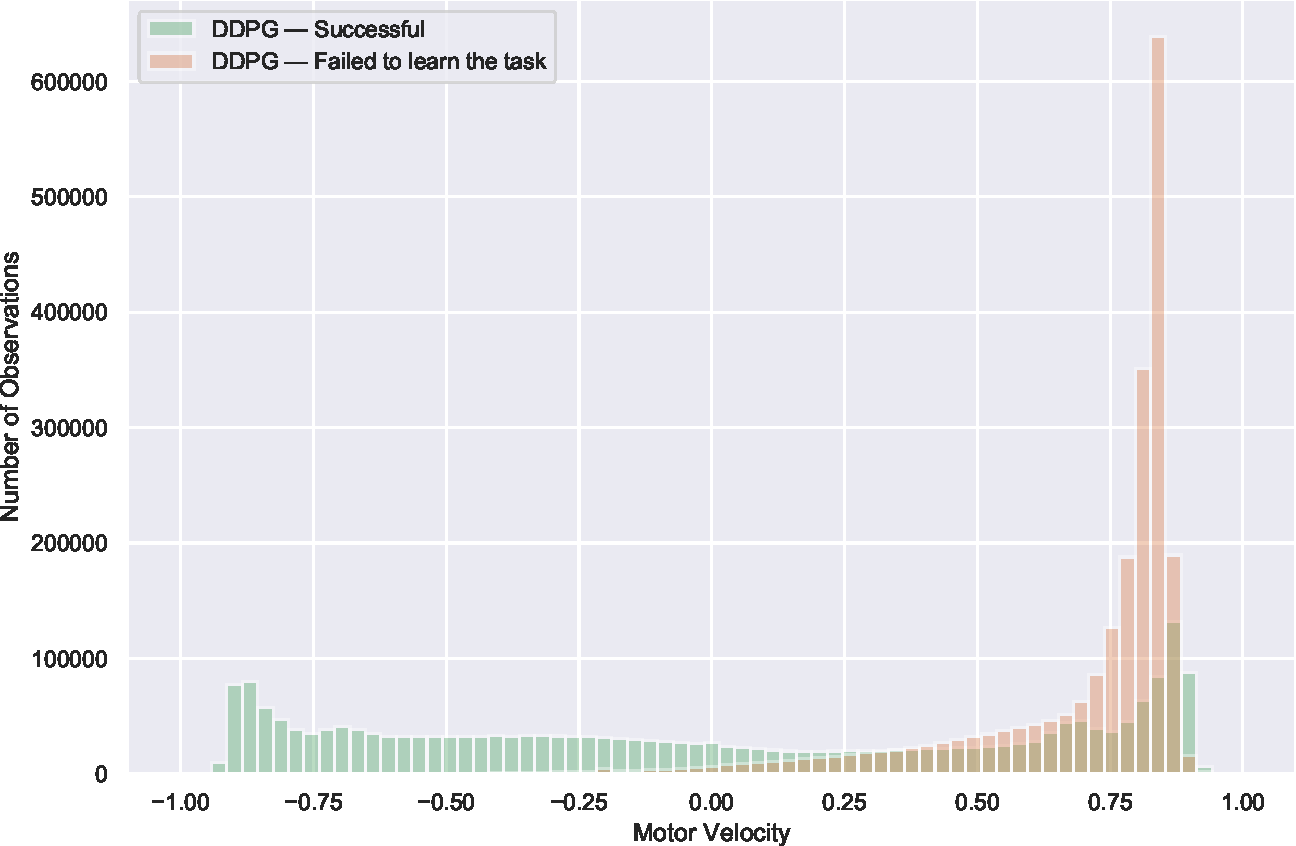
\includegraphics[width=\linewidth]{fig-motor-hist}
    \caption{
        Characterising policy behaviours for the \emph{Move In Direction} task.
        We plot the distribution of motor velocities across many episodes for a successful policy (green) and unsuccessful policy (orange).
        The successful policy learns to pulse the motor in alternating directions (the same strategy used by our heuristic policy).
        In contrast, the unsuccessful policy gets stuck in a local minima where the motor is continuously driven in one direction.
    }
    \label{fig:motor-hist}
\end{figure}

\begin{figure}[ht]
    \centering
    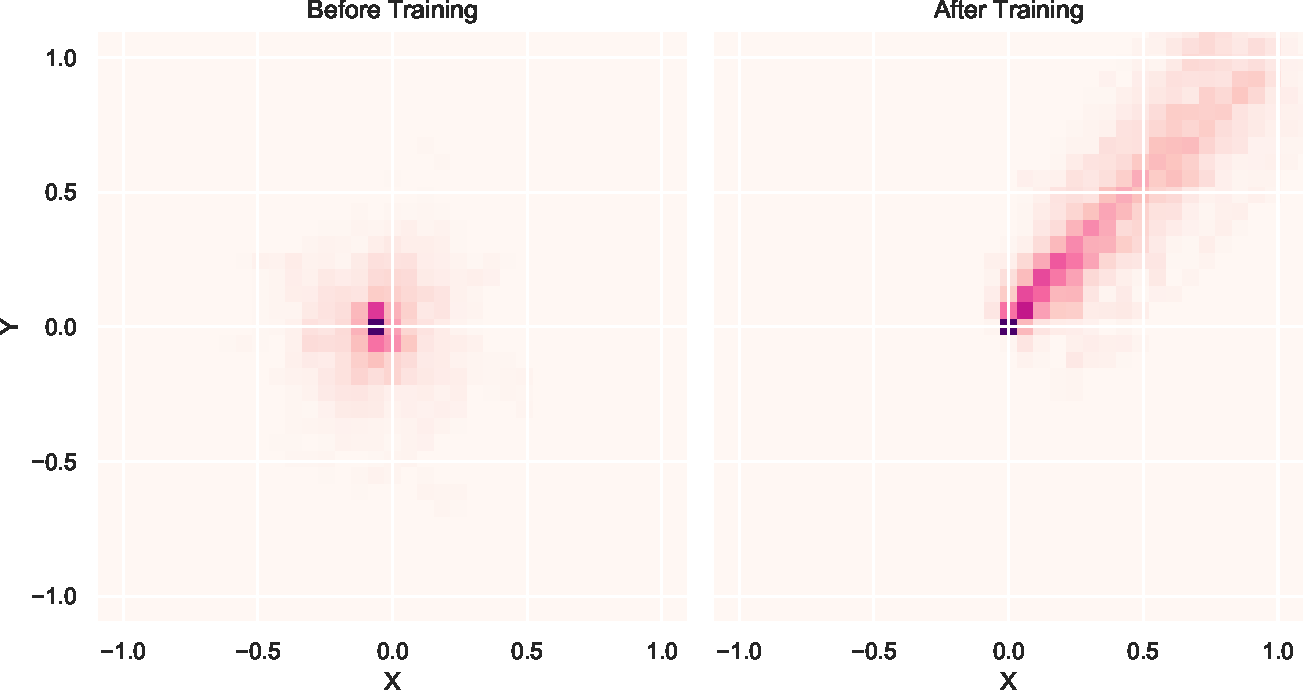
\includegraphics[width=\linewidth]{fig-heatmap}
    \caption{
        Heatmap showing Jitterbug position over 100 episodes before (left) and after (right) training DDPG on the task \emph{Move In Direction}.
        In the second figure, to evaluate the agent, the target direction was fixed at $+45\degree$.
    }
\label{fig:heatmap}
\end{figure}

\subsection{Reduced-Order Training}

\emph{Autoencoder}: The input $X$ is corrupted by adding random noise to each of the features.
Random noise used: $X_\text{noisy} = X + \mathcal{N}(0, 0.1)$.
The autoencoder is fed with the corrupted data $X_{noisy}$ and is trained to reproduce the original data $X$.
Loss used: Mean Squared Error between the output $Y$ and the original data $X$.

Dimensions:
\begin{itemize}
    \item Input/Output: $d = 16$
    \item Latent: several cases - $l = 12,8,4$
\end{itemize}

\emph{Training the Autoencoder}: Gathering of the data used to train the autoencoder: random policy, i.e. an agent was run for 5M steps taking only random actions and each observed state was saved in a file.

Training: from this dataset, 80\% of the data was used to train and 20\% to test.
Use: Once trained, only the encoder part of the autoencoder is used (see figure)

\begin{figure}[ht]
    \centering
    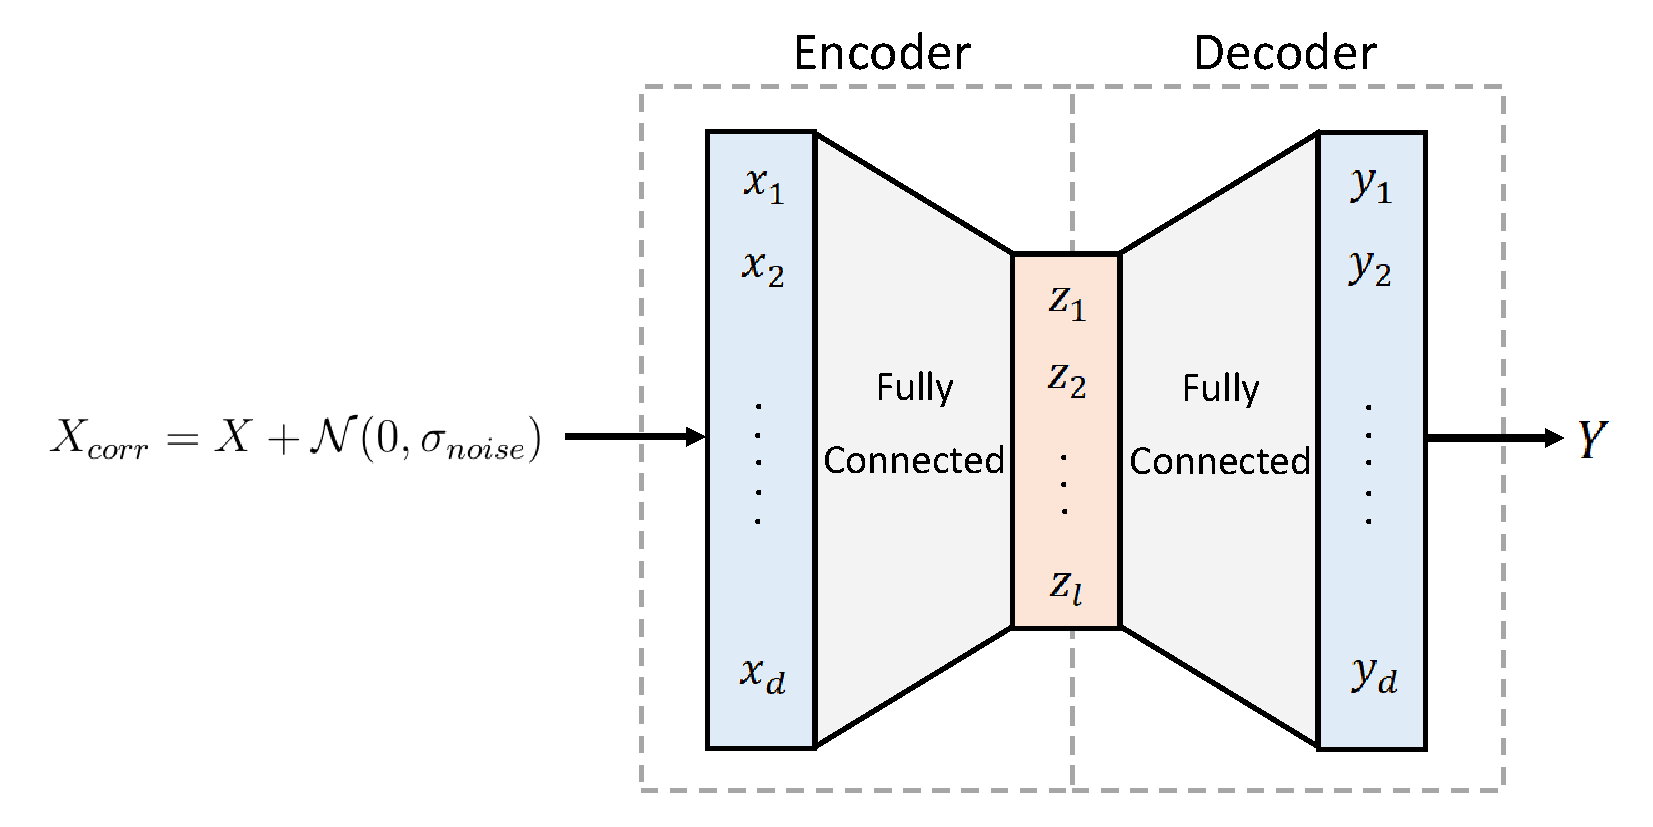
\includegraphics[width=\linewidth]{fig-autoencoder}
    \caption{
        WE used a De-Noising AutoEncoder as a means to learn a reduced-order state representation.
    }
    \label{fig:autoencoder}
\end{figure}

\lipsum[1-7]

\begin{figure*}[p]
    
    \centering
    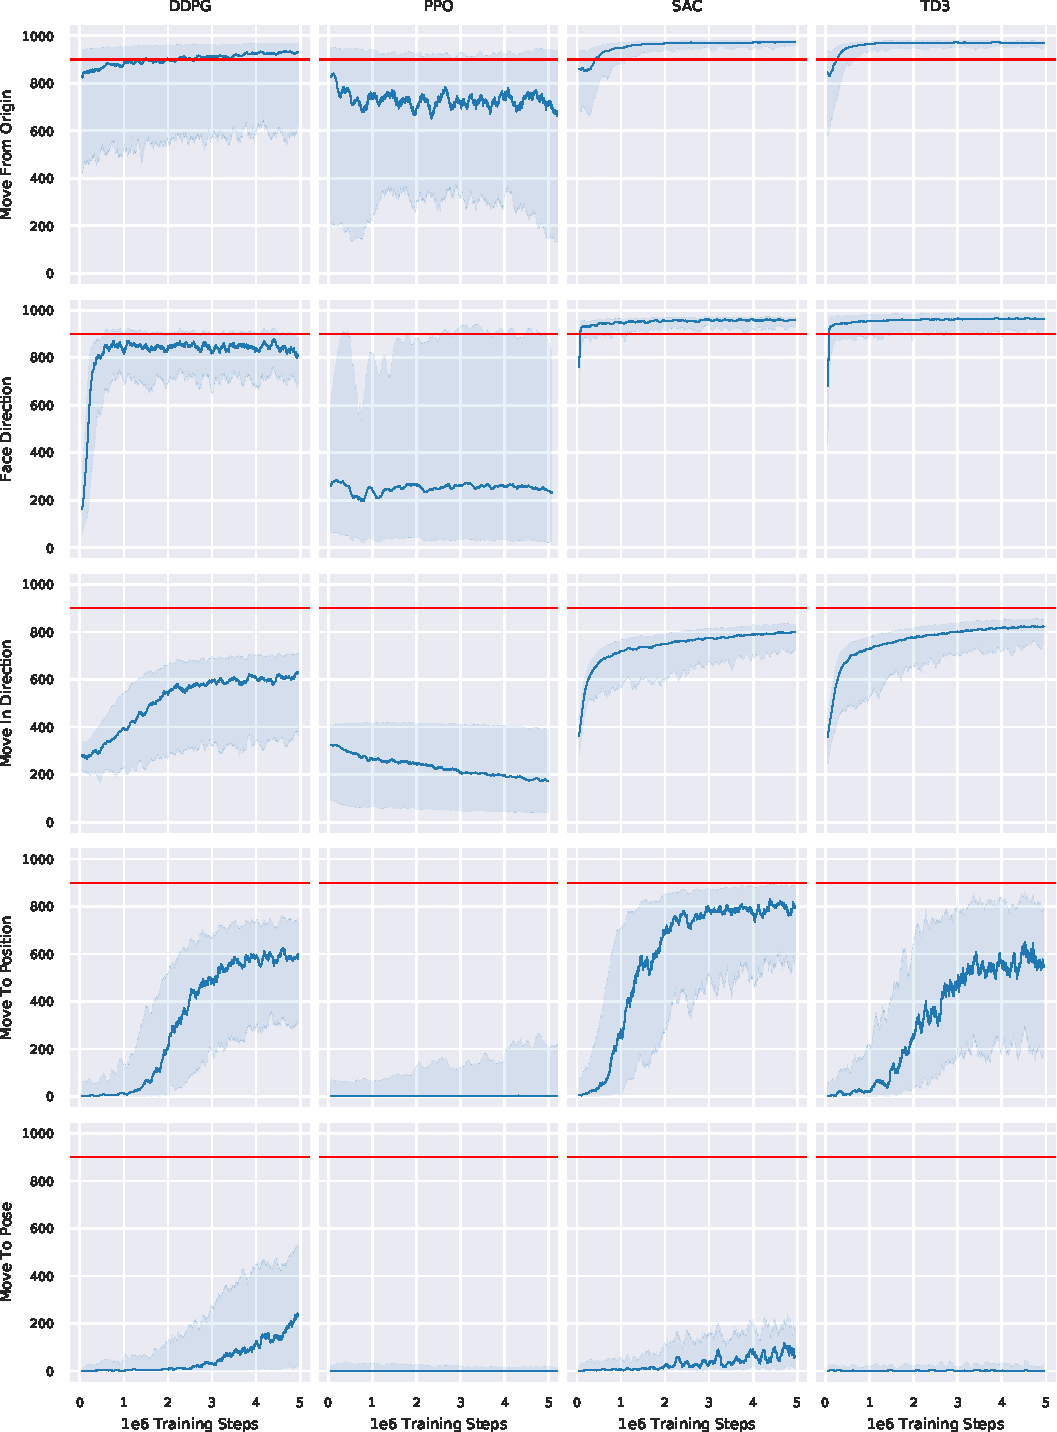
\includegraphics[height=0.94\textheight]{fig-rl-perf}
    
    \caption{
        Characterising the Jitterbug task suite.
        We compare the training progress of DDPG and PPO up to 6 million training steps (6000 episodes).
        We show median (solid line) and the 10\textsuperscript{th} and 90\textsuperscript{th} quartiles (shaded area) of per-episode episode return across 10 random seeds in each figure.
        A task is considered 'solved' if the trained agent consistently scores $\gtrapprox 900$ return per episode (red line).
        All plots are filtered with a 20{\tiny E}\textsuperscript{3} step moving average filter.
    }
    
    \label{fig:rl-perf}
\end{figure*}

\section{DISCUSSION}

\lipsum[1]

\section{CONCLUSION}

\lipsum[1]

%\addtolength{\textheight}{-12cm}   % This command serves to balance the column lengths
                                  % on the last page of the document manually. It shortens
                                  % the textheight of the last page by a suitable amount.
                                  % This command does not take effect until the next page
                                  % so it should come on the page before the last. Make
                                  % sure that you do not shorten the textheight too much.

%%%%%%%%%%%%%%%%%%%%%%%%%%%%%%%%%%%%%%%%%%%%%%%%%%%%%%%%%%%%%%%%%%%%%%%%%%%%%%%%



%%%%%%%%%%%%%%%%%%%%%%%%%%%%%%%%%%%%%%%%%%%%%%%%%%%%%%%%%%%%%%%%%%%%%%%%%%%%%%%%



%%%%%%%%%%%%%%%%%%%%%%%%%%%%%%%%%%%%%%%%%%%%%%%%%%%%%%%%%%%%%%%%%%%%%%%%%%%%%%%%
\section*{APPENDIX}

\lipsum[1]

\section*{ACKNOWLEDGMENT}

We thank Dr. Hanna Kurniawati at the ANU Robust Decision-making and Learning Laboratory for discussions and simulation assistance.  This research was partly supported by an Australian Research Council Discovery Project (DP160100714).  A. Snoswell is supported in part through and Australian Government Research Training Program Scholarship. 


%%%%%%%%%%%%%%%%%%%%%%%%%%%%%%%%%%%%%%%%%%%%%%%%%%%%%%%%%%%%%%%%%%%%%%%%%%%%%%%%

\bibliographystyle{ieeetr}
\bibliography{root}

\end{document}
